\documentclass[11pt,a4paper]{article}
\usepackage[T1]{fontenc}
\usepackage[utf8]{inputenc}
\usepackage{lmodern}
\usepackage{amsmath,amssymb,amsthm,mathtools,mathrsfs}
\usepackage{graphicx,float,xcolor,multicol}
\usepackage[shortlabels]{enumitem}
\usepackage[margin=27mm]{geometry}
\usepackage{microtype,needspace,placeins}
\usepackage{tikz,tikz-cd}
\usetikzlibrary{arrows.meta,calc,positioning,patterns,decorations.pathreplacing}
\usepackage[colorlinks=true,linkcolor=teal,urlcolor=teal,citecolor=teal]{hyperref}
\setlength{\parindent}{0pt}
\setlength{\parskip}{.6em}
\setcounter{secnumdepth}{0}
\allowdisplaybreaks
\raggedbottom
\providecommand{\cross}{\times}
\DeclareUnicodeCharacter{2020}{\ensuremath{\dagger}}
\DeclareMathOperator{\supp}{supp}
\DeclareMathOperator*{\esssup}{ess\,sup}
\providecommand{\chapter}{\section}
\newenvironment{tool}[2]{\subsection*{Tool #1 --- #2}}{}
\newcommand{\ToolRef}[1]{Tool #1}
\newcommand{\FigureTag}[2]{\textit{Figure #1}}
\newcommand{\Result}[1]{\subsection*{#1}}
\newcommand{\Application}[1]{\subsubsection*{Application\if\relax\detokenize{#1}\relax\else\space--- #1\fi}}
\newcommand{\ProofHeading}{\par\textit{Proof.}\space}
\newcommand{\ProofOf}[1]{\par\textit{Proof of #1.}\space}
\newcommand{\RemarkHeading}{\par\textbf{Remark.}\space}
\newcommand{\NoteHeading}{\par\textbf{Note.}\space}
\newcommand{\ExerciseHeading}{\par\textbf{Exercise.}\space}

\graphicspath{{figures/elliptic-curves/}}
\begin{document}
\section*{Elliptic Curves — Harmonic Perspective}
% BLOG-CONTENT-BEGIN
\textbf{III) \underline{Harmonic Perspective}}

Let us begin with a calculation. 

\textbf{Calculation}: We shall first compute the Laurent series of the Weierstrass function,
\begin{center}
    \begin{equation*}
    \begin{aligned}
        \wp_{\Lambda}(z) &= \frac{1}{z^2} + \sum_{\omega \in \Lambda\backslash\{0\}}\bigg[\bigg(\frac{1}{\omega^2}\bigg)\bigg(\frac{d}{d(zw^{-1})}\bigg(\frac{1}{1-zw^{-1}}\bigg)\bigg) - \frac{1}{\omega^2}\bigg] \\
        &= \frac{1}{z^2} + \sum_{\omega \in \Lambda\backslash\{0\}}\bigg(\frac{1}{\omega^2}\bigg(1 + 2zw^{-1} + 3(zw^{-1})^2 +\cdots\bigg) - \frac{1}{\omega^2}\bigg)\\
        &= \frac{1}{z^2} + 3G_4z^2 + 5G_6z^4 + \cdots 
    \end{aligned}
\end{equation*}
\end{center}

Because the series converges absolutely, the odd terms cancel each other. Here 
$$G_{2k} = \sum_{\omega \in \Lambda\backslash\{0\}} \omega^{-2k}$$

Now consider the following Laurent expansions:

\begin{equation*}
    \begin{aligned}
        &\wp_{\Lambda}(z) = \frac{1}{z^2} + \cdots\\
        &\wp_{\Lambda}(z)^2 = \frac{1}{z^4} + 6G_4 + \cdots\\
        &\wp_{\Lambda}(z)^3 = \frac{1}{z^6} + \frac{9G_4}{z^2} + 15G_6 +\cdots\\
        &(\wp_{\Lambda}'(z))^2 = \frac{4}{z^6} - \frac{24G_4}{z^2} - 80G_6 + \cdots\\
    \end{aligned}
\end{equation*}

The cubic in $\wp_{\Lambda}(z)$ given by $a\wp_{\Lambda}(z)^3 + b\wp_{\Lambda}(z)^2 + c\wp_{\Lambda}(z) + d$ has the following Laurent series around $0$,
$$\frac{a}{z^6}+\frac{b}{z^4} + \frac{(9aG)4 + c)}{z^2} + (15aG_6 + 6bG_4 + d) + \cdots$$

If the cubic is to equal $(\wp_{\Lambda}'(z))^2$, by comparing coefficients we must have, 
$$a = 4, b = 0, c = -60G_4, d = -140G_6$$
Set,
$$g_2 = 60G_4 = \sum_{\omega \in \Lambda\backslash\{0\}} \frac{60}{\omega^4}, \text{ and } g_3 = 140G_6 = \sum_{\omega \in \Lambda\backslash\{0\}} \frac{140}{\omega^6}$$

to get, 
\begin{equation*}
    \begin{aligned}
        (\wp_{\Lambda}'(z))^2 &=  4\wp_{\Lambda}(z)^3 - g_2\wp_{\Lambda}(z) - g_3\\
        &= 4(\wp_{\Lambda}(z)-e_1)(\wp_{\Lambda}(z)-e_2)(\wp_{\Lambda}(z)-e_3) 
    \end{aligned}
\end{equation*}

The constants $g_2$, $g_3$, and more generally $G_{2k}$ occur naturally for every elliptic curve parametrized by a lattice. Regard them as functions of the lattice expressed through its generators $\omega_1$ and $\omega_2$. They then satisfy:
\begin{equation*}
    \begin{aligned}
        &G_{2k}(\mu\Lambda) = \sum_{\omega \in \mu\Lambda\backslash\{0\}}\frac{1}{\omega^{2k}} = \mu^{-2k}G_{2k}(\Lambda)  \text{      (seen as functions of }\Lambda)\\
        &G_{2k}(\mu\omega_1, \mu\omega_2) = \mu^{-2k}G_{2k}(\omega_1, \omega_2)  \text{ 
     (seen as functions of generators)}\\
    \end{aligned}
\end{equation*}

Note, $G_{2k}(\omega_1, \omega_2) = \omega_2^{2k}G_{2k}(\omega_1/\omega_2, 1)$. If we let $f(\omega_1/\omega_2):= G_{2k}(\omega_1/\omega_2, 1)$, then $f$ must be independent of the choice of a basis for $\Lambda$. Hence $f$ must satisfy some symmetries. If $M = \begin{pmatrix}
    a&b\\c&d 
\end{pmatrix}\in PSL_2(\mathbb{Z})$, the lattice generated by $\omega_1$ and $\omega_2$ is the same as the lattice generated by the vectors $M\begin{pmatrix}
    \omega_1\\ \omega_2
\end{pmatrix}$. So, we must have,
$$\color{red}\omega_2^{2k}f\bigg(\frac{\omega_1}{\omega_2}\bigg) = (c\omega_1+d\omega_2)^{2k}f\bigg(\frac{a\omega_1+b\omega_2}{c\omega_1+d\omega_2}\bigg)$$


Henceforth we shall look at lattices of the form $\mathbb{Z}\oplus\mathbb{Z}\tau$, with $\tau \in \mathbb{H}$. The calculation above motivates the following definition.

\subsection*{Definition 0.1} A meromorphic function $f$ on $\mathbb{H}$ is \textbf{weakly modular of weight $2k$} if it satisfies the following symmetry law: 
$$f(z) = (cz+d)^{2k}f\bigg(\frac{az+b}{cz+d}\bigg)$$

$\forall$ $\begin{pmatrix}
    a&b\\c&d
\end{pmatrix}\in PSL_2(\mathbb{Z})$. A weakly modular function is \textbf{modular} if $f(q)$ is meromorphic at $0$, where $q = e^{2\pi i z}$.


\textbf{Remark.} A natural domain for weight $0$ modular forms is $\mathbb{H}$ up to symmetries of the modular group. The following figure illustrates how these quotient spaces look if one considers the ball model for the hyperbolic space.

\textbf{Remark.} The holomorphicity of $f(q)$ in $q$ is explained here: The exponential map is a covering map of the punctured disk by $\mathbb{H}$, and modular forms are invariant under deck transformations of that cover, since they are integer translations. Therefore, one can evaluate $f$ locally on evenly covered neighbourhoods of the punctured disk. Evidently, this is well-defined.    

Let $v_p(f)$ denote the order of a zero or pole of $f$ at $p$. By $v_{\infty}(f)$ we mean the order of $f(q)$ at $q=0$; that is, if $f(q)=c_{-N}q^{-N}+\cdots$ with $c_{-N}\neq0$, then $v_{\infty}(f)=-N$. With the help of the following lemma we shall yet again compute the moduli space of elliptic curves in a novel way. 


\subsection*{Lemma 0.1}Let $f$ be modular of weight $2k$, then,
$$v_{\infty}(f) +\frac{1}{3}v_{\rho}(f) + \frac{1}{2}v_{i}(f) + \sum_{p} v_p(f) = \frac{k}{6}$$

where $\rho = \frac{1+i\sqrt{3}}{2}$, $p\in \overline{D}/PSL_2(\mathbb{Z})$, and $D$ is the fundamental domain.


\textit{Proof.}
    We shall integrate $df/f$ on the contour below in two distinct ways:

    \begin{figure}[htp]
            \centering
            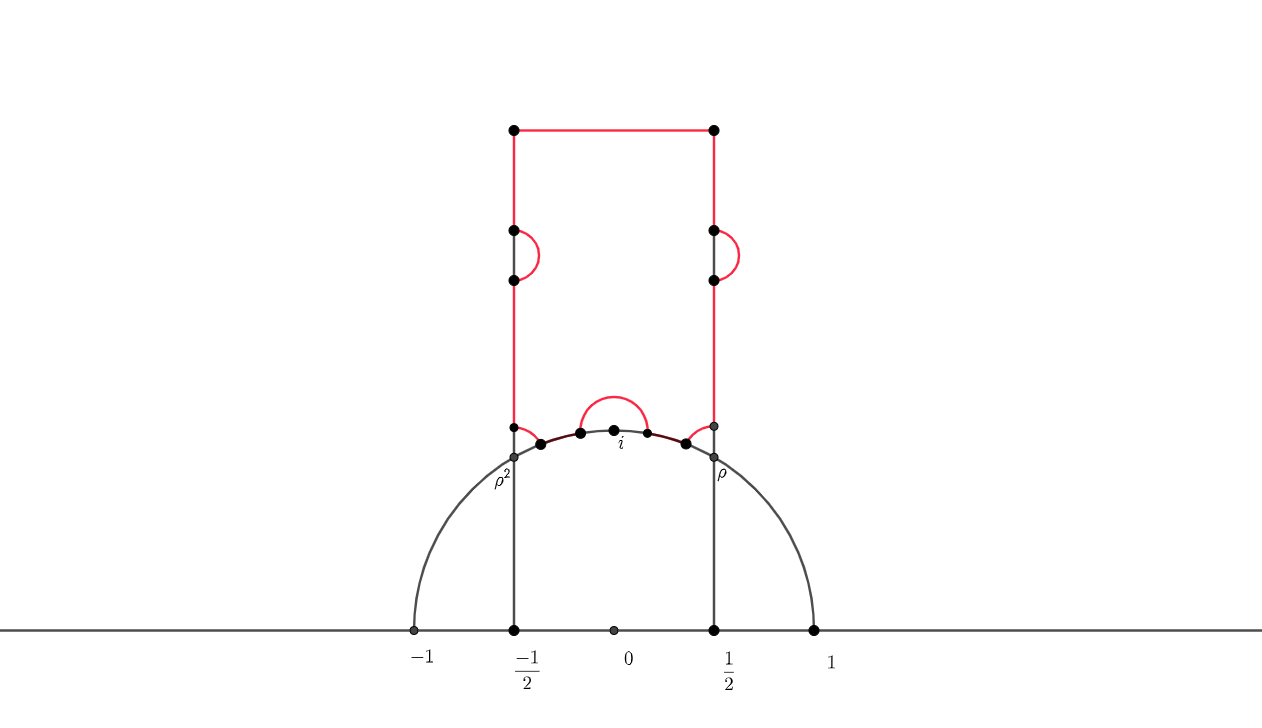
\includegraphics[width=15cm]{Contour.png}
        \end{figure}


By the Argument Principle, 
$$\int_{C}\frac{f'(z)}{f(z)}dz = \sum_{p\neq i, \rho}v_p(f)$$

Let $\beta$ and $\beta'$ be the vertical parts of the contour, and let $\alpha$ be the horizontal segment. Let the bumps around $\rho, \rho^2, i$ be $\gamma_{\rho}, \gamma_{\rho^2}, \gamma_{i}$, and let the remaining portion be $\gamma$. Slash action tells us that $f(z+1) = f(z)$, which implies,
$$\int_{\beta}\frac{df}{f} + \int_{\beta'}\frac{df}{f} = 0$$

The change of variables $z\rightarrow e^{2\pi i z}$ sends the segment $\alpha$ to a circle around $0$, giving 
$$\int_{\alpha}\frac{df}{f} = \int_{\text{exp}(\alpha)}\frac{df(q)}{f(q)} = -2\pi i v_{\infty}(f)$$

Completing the bumps $\gamma_{\rho}, \gamma_{\rho^2}, \gamma_{i}$ to circles $\widetilde{\gamma}_{\rho}, \widetilde{\gamma}_{\rho^2}, \widetilde{\gamma}_{i}$ we note that:
$$\int_{\widetilde{\gamma}_{i}} = 2\pi i v_i(f),  \int_{\widetilde{\gamma}_{\rho}} = 2\pi i v_{\rho}(f),  \int_{\widetilde{\gamma}_{\rho^2}} = 2\pi i v_{\rho^2}(f)$$

Now as, 
$$\int_{\delta_n}\frac{dz}{z} = \frac{2\pi}{n}$$

where $\delta_n$ is the $1/n$ of the of the unit circle; we see that,
\begin{equation*}
    \begin{aligned}
        \frac{1}{2\pi i}\int_{\gamma_{\rho}+ \gamma_{\rho^2}+ \gamma_{i}} \frac{df}{f} &=-\frac{1}{2}v_i(f) - \frac{1}{6}v_{\rho}(f) - \frac{1}{6}v_{\rho^2}(f)\\
        &= -\frac{1}{2}v_i(f) -\frac{1}{3}v_{\rho}(f)\\
    \end{aligned}
\end{equation*}

Finally consider the transform $z\rightarrow -1/z$ that sends $\gamma$ to $\overline{\gamma}$. Note, 
$$df(-1/z) = d(z^{2k}f(z)) = z^2kdf(z) + 2kz^{2k-1}f(z)dz$$

which gives, 
$$\frac{df(-1/z)}{f(-1/z)} = \frac{z^{2k}df(z)}{z^{2k}f(z)} + 2kz^{2k-1}\frac{f(z)dz}{z^{2k}f(z)} = \frac{df(z)}{f(z)} + 2k\frac{dz}{z}$$

Therefore, 
$$\int_{\overline{\gamma}}\frac{df(-1/z)}{f(-1/z)} = \int_{\overline{\gamma}}\frac{df}{f} + \int_{\overline{\gamma}}2k\frac{dz}{z} = -\int_{\gamma}\frac{df}{f} + 2k\int_{\overline{\gamma}}\frac{dz}{z}$$
implying, 
$$\int_{\gamma} \frac{df}{f} = k\int_{\overline{\gamma}}\frac{dz}{z}$$

Now as the bumps tend to $0$, the integral on the right-hand side approaches $k/6$ (as $\gamma$ would approach $1/6$th of the unit circle) giving us,

$$\frac{1}{2\pi i}\int_{C}\frac{df}{f} = -v_{\infty}(f) - \frac{1}{3}v_{\rho}(f) - \frac{1}{2}v_{i}(f) + \frac{k}{6}$$

(Keep track of the orientations to get the correct signs.)


\subsection*{Theorem 0.3}
    "The moduli space of elliptic curves is isomorphic to the Riemann sphere."


\textit{Proof.}
    Define, 
    $$j:\mathbb{H} \rightarrow \mathbb{CP}^1$$
    $$j(z) := \frac{g_2^3(z)}{g_2^3(z) - 27g_3^2(z)}$$

where (recall) $g_2(z) = 60\sum(nz+m)^{-4}$ and $g_3(z) = 140\sum(nz+m)^{-6}$ are holomorphic on $\mathbb{Z}$. Note that, $g_2(\infty) = \frac{4}{3}\pi^4$, $g_3(z) = \frac{8}{27}\pi^6$, so $\Delta(z):= g_2^3(z) - 27g_3^2(z)$ vanishes at $\infty$. Applying the lemma above to $\Delta$ yields,
$$\frac{6}{6} = v_{\infty}(\Delta) +\frac{1}{3}v_{\rho}(\Delta) + \frac{1}{2}v_{i}(\Delta) + \sum_{p} v_p(\Delta)$$

$\Delta$ being holomorphic and $v_{\infty}(\Delta) \geq 1$ implies $v_{\infty}(\Delta) = 1$. Also, as $g_2(\infty) \neq 0$, $j(z)$ has a simple pole at $\infty$. Now, applying the lemma to $g_3^2 - \lambda\Delta$ (which is again holomorphic, even at infinity) yields,
$$\frac{6}{6} = v_{\infty}(g_3^2 - \lambda\Delta) +\frac{1}{3}v_{\rho}(g_3^2 - \lambda\Delta) + \frac{1}{2}v_{i}(g_3^2 - \lambda\Delta) + \sum_{p} v_p(g_3^2 - \lambda\Delta)$$

implies, 
$v_{\infty}(g_3^2 - \lambda\Delta) = 1$, or $v_{i}(g_3^2 - \lambda\Delta) = 2$, or $v_{\rho}(g_3^2 - \lambda\Delta) = 3$, or $v_p(g_3^2 - \lambda\Delta) = 1$. In each case, $j(z) = \lambda$ has a unique solution modulo the action of the modular group. 

\textbf{Remark.} $j(z)$ being a weight $0$ modular form factors through $D/PSL_2(\mathbb{Z})$. For each $\lambda$ in the fundamental domain one has a unique class of elliptic curves $[\mathbb{C}/\Lambda_0, [\Lambda_0]]$, and $j$ maps that to $\mathbb{C}$. In other words, to each equivalence class of elliptic curves $j$ associates an invariant. This function is called the $j$-invariant in the literature. Said differently, two elliptic curves $E_1, E_2$ are isomorphic iff $j(E_1) = j(E_2)$.


\textbf{Remark.} Note that $j(\infty) = \infty$. If one considers the elliptic curve corresponding to $\lambda = \infty$, one can convince oneself that it is the infinite cylinder. This compactifies the moduli space of elliptic curves to a genus-$0$ surface.

We shall end by stating how the harmonic perspective fits in among the other two natural-seeming ones. Let $E: y^2 = 4x^3 - g_2x - g_3$ be an elliptic curve with $g_2, g_3 \in \mathbb{Z}$, and $\Delta \neq 0$. Define,
$$a_p(E) = p - \#\{\text{integer solutions to $E$ modulo $p$}\}$$

for a prime $p$. In the 1950s, Taniyama conjectured that for such curves there is a modular form,
$$f(\tau) = \sum_{n = 0}^{\infty}a_n(f)e^{2\pi i \tau}$$

such that,
$$a_p(f) = a_p(E)$$

for all primes $p$. Later, For an odd prime $p$ and a triple $(a,b,c)$ satisfying $a^p+b^p=c^p$, Frey constructed the elliptic curve
$$y^2 = x(x-a^p)(x+b^p)$$

and conjectured that these curves wouldn't be modular in the sense described above. Ribet and Serre proved Frey's conjecture, and the final blow was delivered by Andrew Wiles and Richard Taylor by proving Taniyama's conjecture (now known as \textbf{Modularity Theorem}), thereby also proving \textbf{Fermat's Last Theorem}!
% BLOG-CONTENT-END
\end{document}
